%% *************************************************************************
%%
%% This is a derivative work of the RIT Space Exploration Standard defining 
%% guidelines for content and formatting of project design documents.
%%
%% This document uses IEEEtran.cls, the official IEEE LaTeX class
%% for authors of the Institute of Electrical and Electronics Engineers
%% (IEEE) Transactions journals and conferences.
%%
%% *************************************************************************

%% *************************************************************************
% LaTeX REFERENCES
% ----------------
%   Intro to LaTeX: http://www.rpi.edu/dept/arc/docs/latex/latex-intro.pdf
%   Comprehensive LaTeX symbol list: http://tug.ctan.org/info/symbols/comprehensive/symbols-a4.pdf
%% *************************************************************************

% tell \LaTeX what kind of formatting to use
\documentclass[conference]{IEEEtran} % http://www.ctan.org/pkg/ieeetran
\usepackage{blindtext} % enable placeholder text generator
\usepackage{graphicx} % enable toolbox for embedding figures and pictures
\usepackage{nomencl} % enable package for adding a list of variables and constants at the beginning, aka "nomenclature"
\usepackage{siunitx} % enable package for easily formatting units
\usepackage{hyperref} % enable package for cross-referencing figures, sections, references etc.
% how to use hyperref: http://www2.washjeff.edu/users/rhigginbottom/latex/resources/lecture09.pdf
\usepackage[T1]{fontenc} % change text encoding to make it more crisp
\usepackage{etoolbox} % enable conditionals for help text
\usepackage{booktabs} % make beautiful tables!
\usepackage{tabularx}

% initialize nomenclature package
\makenomenclature{}

% set title. choose something as descriptive and precise as possible. Descriptive > sounding cool. remember this!
\title{Design and Fabrication of an Environmental Testing Chamber for Simulating Space-like Vacuum and Thermal Conditions}


\author{
  % List the authors of the design document. The Champion should go first.
  % The \$~\$ markers tell \LaTeX{} to treat the text inside to be treated as a math expression. This way you can use operators like \textcaret{} to place characters as superscripts.
  % Some \LaTeX{} templates handle the author block in different ways. For example, the \href{http://www.worldscientific.com/worldscinet/jai}{Journal of Astronomical Instrumentation} requires the authors' addresses and emails to be included as well.
  % The \textbackslash{}thanks command puts the contents inside those brackets in a footnote at the bottom of the first page. Technically speaking, \textbackslash{}thanks is just a specially formatted footnote.
  % IEEE also has a ``long form'' author block for many authors. Check here for more information:
  % \url{https://tex.stackexchange.com/questions/156523/multiple-authors-with-common-affiliations-in-ieeetran-conference-template}
  % Read here for a more advanced options to modifying footnotes in the author block:  \url{http://tex.stackexchange.com/questions/826/symbols-instead-of-numbers-as-footnote-markers}
  %   Here, we use the IEEE long-form author block.
  \IEEEauthorblockN{% This block is for author Names.  %the number in the bracket is a reference number to identify this footnote. \LaTeX will figure out what symbol to put there.
    T.J.~Tarazevits\IEEEauthorrefmark{1},
  }
  \IEEEauthorblockA{% This block is for the author Affiliations, aka department and university
    RIT Space Exploration, Rochester Institute of Technology \\ %\\ starts a new line
    Rochester, N.Y. \\
    Email:
    \IEEEauthorrefmark{1}tjt3085@rit.edu,
  }
  %%   Below, we use the short-form author block and basically hack it to suit our needs.
  % Philip~Linden$^{*\dagger}$%
  %   \thanks{$^{*}$Project Champion}%
  %   \thanks{$^{\dagger}$BS/MEng '17, Mechanical Engineering},
  % Austin~Bodzas$^{\ddagger}$%
  %   \thanks{$^{\ddagger}$BS '19, Computer Science},
  % Drew~Walters$^{\S}$%
  %   \thanks{$^{\S}$BS '18, Mechanical Engineering Technology},
  % T.J.~Tarazevits$^{**}$%
  %   \thanks{$^{**}$BS '19, Game Design \& Development}%

  %%   If there are many authors, consider using symbolic, numeric (aka arabic),  alphabet footnotes or a combination thereof.
  %% the recommended order for symbolic footnotes is
  %%   (1) asterisk        *   *
  %%   (2) dagger          †   \dagger
  %%   (3) double dagger   ‡   \ddagger
  %%   (4) section symbol  §   \S
  %%   et cetera. For higher counts, use 2x symbols (1)-(4) (i.e. (5) two asterisks **). Keep cycling through (1)-(4) using 3x, 4x, and so on.
  %%   Note that these symbol codes work in math mode and text mode.
  %%   There are ways to make LaTeX do this for you, but it is more advanced and not entirely necessary, especially for short author lists. Not worth the hassle, in my opinion.
}
% page header for pages other than cover page
\markboth{Environmental Test Chamber PDD}%
{Linden \MakeLowercase{\textit{et al.}}: RIT Space Exploration}

% Initial setup is over, start building the document itself
\begin{document}
\maketitle%
% correct bad hyphenation here, separated by spaces
\hyphenation{explor-ation}

\begin{abstract}
  This proposal describes a project to build a controlled thermal vacuum chamber, called an Environmental Test Chamber or ETC, as well as associated test automation software, and documentation describing its safe operation and use by other SPEX teams. Low-cost pumps and off the shelf hardware enable useful vacuum to be generated. Vacuum pumps under \$200 have been shown to achieve up to -28 inHG. While this is not an accurate representation of the space environment, these vacuum conditions are suitable for High Altitude Balloon component testing, and other flight hardware. \cite{vacChamberExp}

      % The abstract is a brief summary of the design document. Typically it includes the purpose of the design document, key goals or objectives, and justifications.
      % Be sure not to confuse the abstract with the introduction.
      % It is easiest to write the abstract after the rest of the paper has been written.
      % That way you can choose key information from the sections that you've already completed and string them together in the abstract.
      % Consider the abstract to be your elevator pitch to anyone reading this design document.
      % What are they reading?
      % What is the goal?
      % Why is it worth my time?
      % The abstract is what will show up in Google results and other search engines, and what people will read when they are deciding what is worth their time and brain power.
\end{abstract}

\label{sec:nomenclature}
\newcommand{\nomunit}[1]{%
\renewcommand{\nomentryend}{\hspace*{\fill}#1}}
\renewcommand{\nompreamble}{
    % If you include mathematical expressions or express variables in the design document, list them with their corresponding definitions here as a list.
    % The two lines below make it look nice when defining units/values to constants.

    % Note that math terms and non-math terms are separated and alphabetized, regardless of the order in which they are defined. (Recall terms \$like this\$ are in the math environment)
    % Read more about advanced nomenclature formatting here:\\
    % \url{https://www.sharelatex.com/learn/Nomenclatures}
  }
\nomenclature{RIT}{Rochester Institute of Technology}
\nomenclature{SPEX}{RIT Space Exploration}
\nomenclature{PDD}{Project Design Document}
\nomenclature{ETC}{Environmental Test Chamber}
% Below are examples of using nomenclature for math symbols and constants or units
\printnomenclature{}


% HELPFUL HINT: If you get the warning ``Command terminated with space.'' when using a \command try placing ``%'' or ``{}'' immediately following the command.

% The sections included here are required. Additional sections and subsections may be added as necessary.
\section{Introduction}
\label{sec:introduction}
  % The introduction is a place to give background and context before diving into the subject matter.
  % Establish context for the work you are about to propose and the main ideas of the proposition itself.

\IEEEPARstart{S}{pace} provides a unique and challenging engineering environment.
Hardware designed to operate in this environment needs to be validated in realistic testing conditions before flight.
An Environmental Test Chamber (ETC) provides a controlled test bed for simulating the atmospheric and thermal environment of space and near-space environments that can be repeated at low cost.
RIT does not have readily available and suitable ETCs for student use.
Some laboratories have expensive vacuum pumps but are unwilling to allow unsupervised use by students or testing of unproven engineering designs.
For example, space-qualified thermal vacuum chambers built by other universities can cost over \$5,000 for the vacuum pump alone.\cite{teb13}
Low cost, commercial vacuum pumps provide the opportunity to achieve relatively low pressures in a small testing volume for dramatically lower cost.
DIY vacuum chambers are a relatively popular project for amateurs on Youtube and other online forums.\cite{korYoutube}

\section{Primary Objective}
\label{sec:primary-obj}
  % At the end of the day, whether the project ``succeeds'' or ``fails'' is judged against the objectives it sought to meet.
  % Note that results that contradict expectations/hypotheses are not failures if the scientific \& engineering methods are followed along the way.
  % Sometimes our expectations are wrong and that can be just as successful as getting data we thought we'd see.
  % What matters are what questions you intend to answer.
  % This is the main purpose or main goal the project hopes to achieve.

  The goal of this project is to design, build, and verify a functioning ETC that enables testing of flight components and flight systems in a controllable thermal and low pressure environment.
  Students will research the expected environmental conditions of high altitude flight and the on-orbit environment.
  Using low cost components, students will construct an ETC that can replicate those environments within a reasonable degree.
  Accuracy in simulation will be traded for reduced cost.
  The final ETC should have a usable testing volume for hardware SPEX expects to fly in the near term.
  Sensor and computers should be included in the system to enable monitoring the environmental conditions within the chamber, as well as enabling long-duration test cycles across a range of conditions.

% \section{Secondary Objectives}
% \label{sec:secondary-obj}
% Secondary Objectives are lower priority or bonus objectives that are significant but not the main focus of the project. This template does not have secondary objectives.

\section{Benefit to SPEX}
\label{sec:benefit}
% One of the core values of SPEX is to provide opportunities for academic and professional growth for its members,
% and to challenge them with interesting projects.
% In this section, explain how the project would benefit SPEX members as students,
% space enthusiasts, and young professionals.

Proper and thorough testing is a critical component of mission success. Many SPEX projects are unable to test their designs in proper environmental conditions, meaning flight tests assume additional risk. An ETC would enable risk reduction on projects like HAB and IREC, as well as provide opportunities to replicate industry-standard testing on space-like designs.\@

Some examples of near-term testing benefits include HAB camera shutdown investigation. HAB-CV camera performance, IREC desert heat validation, and \$50Sat orbital thermal cycling. Sensors and electronics have performance curves related to environmental conditions. An ETC would enable fine characterization of these sensors before flight, increasing confidence in the data collected.\@

An ETC would have reduced mission risk for each of those projects and will be useful for future iterations of those types of projects. An ETC would likely prove useful to many other applications in the near to medium future.


% Below I have used subsections to identify key ideas in this section. These particular subsections are not required as part of the SPEX Standard, but serve as an example of using subsections in a text.

\section{Implementation}
\label{sec:implementation}
  % What path do you anticipate the project to take?
  At the end of the project, a working Environmental Test Chamber should be delivered. It should be capable of maintaining a near-vacuum for extended periods of time, as well as cycling between 0 and > -25 inHG at reasonable rates (< 1 hour duty-cycle).
\subsection{Deliverables}
\label{subsec:deliverables}
  % When all is said and done, what will you have to show for it?
  % Examples: Hardware, software, poster, ImagineRIT demo, presentations, technical papers...
  The chamber should also be able to subject the test article to thermal variations between -20 C and 50 C. Cooling is considered an advanced feature due to the difficulty of removing thermal energy from the ETC compared to adding thermal energy. 

  An additional feature would be the ability to direct the applied thermal energy to simulate satellite tumbling or orbital cycles. Another metric to consider is the ability to apply the average solar radiation ( 1,368 W/m2) to the working surface of the test article to simulate on-orbit thermal conditions.

  Along with the ETC hardware, there should be a control system allowing for software control of pressure and temperature, as well as data recording and real-time monitoring of the current environment. Users should be able to define preset environmental conditions that the ETC should attempt to maintain within reasonable bounds. Also users should be able to define a test sequence, which may consist of a number of environmental conditions varying over time, as well as the ability to cycle between high and low values for controlled environmental conditions. These should be repeatable N times or for a preset time period. A stretch goal should be to determine the temperature and pressure rates of change for the system, and if possible, determine ways to adjust these rates.

  Finally, detailed operating instructions should be written and validated, to provide a safe way for other members to utilize the ETC. Instructions on setup, operation, maintenance, as well as detailed safety procedures in case of an accident or malfunction should be written and tested with the final hardware.

\subsection{Milestones}
\label{subsec:milestones}
  % Be as detailed as you can, but it's okay if there are unknowns.
  % At the very least, specify how many semester you expect the project to take until it reaches completion.
  This list is preliminary and should be considered a placeholder to be refined during the review process. Times are approximate.

  \begin{table}[hb!]
    % this table is too wide for the two-column format, so we let it expand across both columns
    % we haven't told LaTeX where to put this so it'll find the best place.
        \caption{Notional Timeline of Project Milestones}
        \centering
        \begin{tabularx}{\linewidth}{lX}
            % READ THIS!! https://www.inf.ethz.ch/personal/markusp/teaching/guides/guide-tables.pdf
            \toprule % line on top external edge of table
            % Separate cells in a row with &, move to the next row with \\
            Phase & Task  \\
            \midrule % line separating two internal rows
            1 & Students research the particular variables of the near-space and space environment. The requirements for test article dimensions and usability are determined. \\
            2 & Mechanisms for controlling temperature and pressure and researched and proposed. \\
            3 & Initial design work begins on the mechanical system. Students research materials and component selection, including unorthodox sources like craigslist, to meet requirements. \\
            4 & Initial Assembly begins. Software and sensors are introduced to begin characterizing the responsiveness of the chamber. \\
            5 & Students work to automate control of ETC temperature and pressure. \\
            6 & Dry(empty) testing occurs to validate ETC meets minimum performance requirements. \\
            7 & First component test occurs while software automation continues to be refined. Procedure writing begins. \\
            8 & Full procedure writing finishes alongside completion of automation software. Long duration automated tests are attempted to verify the design. \\
            9 & Remaining time can be dispersed across real testing of flight components, improvements to hardware, software, and procedures as more tests are conducted, as well as completion of the final Technical Report \\
            % LaTeX doesn't really like multi-line cell contents. Try to keep the text in each cell concise!
            \bottomrule
        \end{tabularx}
    \label{tab:timeline1}
    \end{table}

% A notional timeline is shown in \autoref{tab:short-example}.

%\begin{table}[hb!]
%    % the "h" in these brackets tells LaTeX to put the table Here. Try [t] for top and [b] %for bottom,
%    % or [hbp] for "here, or if you can't do that put it at the bottom of the page, or if you %can't do that put it on its own page.
%    % Here we've also used an "!" to yell at LaTeX to DO THIS OR ELSE!
%    \caption{Notional timeline of Project Milestones.}
%    \centering
%    \begin{tabular}{@{}cll@{}}
%    % the letters here ^^^^ designate the columns.
%    % (l=left align, c=center, r=right align)
%    % the weird @{} thingies tell LaTeX to not have left-right padding between cells
%    % so cells butt up right against the edge
%    \toprule
%    Phase & Task & Duration \\
%    \midrule
%    1 & Review existing designs and materials & 2 weeks or less\\
%    2 & Subsystem development & 6 weeks \\
%      & Order PCB design and/or assembly & 6 weeks \\
%      & Review changes and order materials & 2 weeks or less\\
%      & Testing of individual subsystems & 2 weeks \\
%    3 & System assembly & 1 week  \\
%    4 & System testing & 2 weeks  \\
%    5 & Generate documentation and delivery to SPEX & 1 week  \\
%    \bottomrule
%    \end{tabular}
%\label{tab:short-example}
%\end{table}

\section{Externalities}
  % Things not directly related to the work or outcomes, but related to the project as a whole.
\subsection{Prerequisite Skills}
  % Which skills do team members need to have before work can start (not including skills that will be learned ``on the job'')?
  This project does not require advanced machining or analysis skills on the engineering side. Commercial Off the Shelf (COTS) components should be sought out for the pump, electronics, and ETC chamber volume.
  Knowledge and desire of coding will be required to write basic control software. If advanced CS skills are available, more complex control algorithms like PID can be implemented to the automation software.
  Upperclassmen engineers should be available to provide guidance and mentorship on the space environment, safety best practices, and the thermodynamics involved in the ETC.
  

\subsection{Funding Requirements}
  % Estimate costs that would be needed to meet objectives.
  Precision in simulating the space environment should be traded whenever possible to maintain reasonable costs. There are many examples of basic vacuum chambers and ETCs being constructed for low cost using COTS components. The estimated cost of the project should not exceed \$400. Commercial vacuum pumps suitable for this project can be found for under \$100. Similiar vacuum pump projects had total Bill of Material costs including pumps, pressure vessels, and fittings for less than \$250. \cite{vacChamberExp} The use of repurposed components may enable increased functionality while staying under the cost cap.

\subsection{Faculty Support}
  % Identify faculty that will be involved (or would need to be involved) to meet objectives.
  % Note that if a professor is the Principal Investigator (P.I.) for a project, there still needs to be a student as the SPEX Project Champion.
  No faculty have signed on to support this project at this time. It would be wonderful if a faculty member had interest in using the finished product for their own non-critical testing and could offer mentorship and advisement. It is not required for project success.

  The project team should meet or exceed any safety requirements imposed by RIT Environmental Health and Safety

\subsection{Long-Term Vision}
\label{sec:vision}
The ETC enables better testing and validation of SPEX projects. As these projects increase in cost and complexity, accepting the risk of no environmental testing becomes increasingly unadvisable. A fully functional and safe ETC would increase project success and provide data to aid in engineering analysis and validation.

\section*{Acknowledgements}
The author would like to thank Dr.~Bill Destler and Rebecca Johnson for being exemplary %humans, Anthony Hennig for founding RIT Space Exploration, and all the SPEX members that %continue to invest their time and energy into the pursuit of space exploration.

\bibliographystyle{IEEEtran}
\bibliography{etc}

%\onecolumn
%\appendices{}
%\section{Project Life Cycle}
%\begin{figure}[h]
%  \centering
%  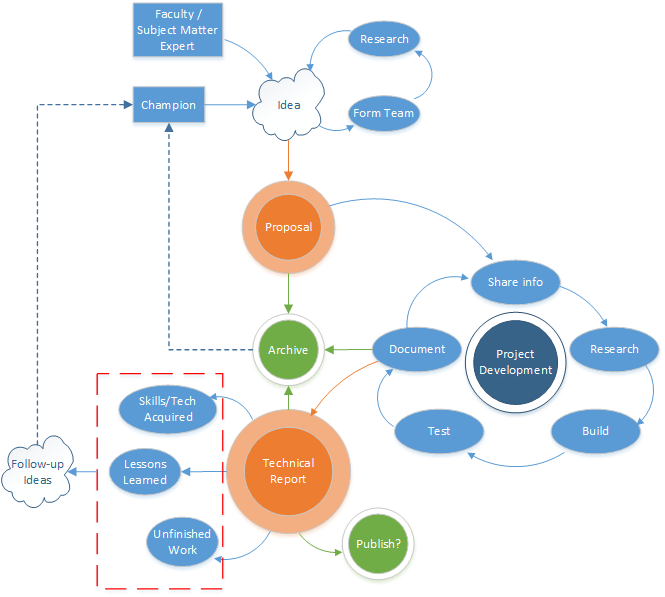
\includegraphics[]{figs/project-life-cycle.png}
%  \caption{Enlarged version of the diagram in \autoref{fig:lifecycle}.}
%\end{figure}

\end{document}
